\documentclass[journal]{IEEEtran}

\usepackage{amsmath,amssymb}
\usepackage{amsthm}
\newtheorem{proposition}{Proposition}
\newtheorem{corollary}[proposition]{Corollary}
\usepackage{graphicx}
\usepackage{booktabs}
\usepackage{algorithm}
\usepackage{algpseudocode}
\usepackage{url}
\usepackage[hidelinks]{hyperref}
\usepackage{siunitx}
\sisetup{group-separator={,},group-minimum-digits=4}

\graphicspath{{figures/}}

\newcommand{\social}{\textsc{Social}}
\newcommand{\permcontrol}{\textsc{Perm}}
\newcommand{\polcontrol}{\textsc{Rand}}

\begin{document}

\title{Does the Score Do the Work? Permutation Controls for\\
Score-Weighted Metaheuristics}

% Author block withheld in the public copy. Fill in before submission.
\author{Anonymous Author%
\thanks{Manuscript prepared \today.}}

\markboth{IEEE Transactions on Evolutionary Computation}%
{Permutation Controls for Score-Weighted Metaheuristics}

\maketitle

\begin{abstract}
Many population-based optimizers weight interactions by a per-neighbour
score---a centrality on the population graph, the quality of a neighbour's
best---on the claim that the score identifies informative agents. The usual
evidence is an ablation, which cannot establish that claim: deleting the
weighting changes the mixing operator as well as the information it carries,
so any difference is equally consistent with the weights having been merely
unequal. We separate the two by permuting the score across nodes, which leaves
the mechanism at full strength and destroys only the correspondence between a
node's position and its weight. We prove this control equals uniform mixing in
expectation while retaining the original's weight heterogeneity pathwise, and
bound when such a comparison is informative at all. A second control randomises
an adaptive component's selection rule. On a published betweenness-weighted
small-world optimizer the mechanism proves active---displacing each update by a
third of the population's spread---and uninformative: over $104$ function
comparisons on two suites, three dimensions and five budgets, permutation
changes nothing that survives correction. Unchanged, the same instrument
returns a uniformly beneficial effect on one further mechanism, a uniformly
harmful one on another, and---on a second published optimizer, the fully
informed particle swarm---a quality weighting whose per-function effects reach
$|\delta|=1$ in \emph{both} directions and cancel in the mean. The null is
therefore a property of the mechanism, not of a test without power. The last
case also carries a methodological lesson: a suite average alone calls it and
the centrality null the same thing, while per-function correction alone hid a
real effect in our own adaptive scheme, so both views are needed. Separating
the properties an ablation confounds shows unequal weights help on $3$ of $28$
functions while the assignment helps on none, so betweenness---about $30\%$ of
runtime---can be replaced by any heterogeneous weighting at no cost.
\end{abstract}

\begin{IEEEkeywords}
Metaheuristics, ablation studies, experimental methodology, swarm
intelligence, network topology, reproducibility.
\end{IEEEkeywords}

\IEEEpeerreviewmaketitle

\section{Introduction}
\label{sec:intro}

A large class of population-based optimizers is justified by a score. Candidate
solutions are placed on a graph, a per-neighbour quantity is computed---a
centrality of the graph, the quality of a neighbour's best---and the update is
weighted so that agents learn preferentially from the neighbours the score
distinguishes. The accompanying argument is causal: the method performs well
\emph{because} the score identifies informative agents. Where such mechanisms
are evaluated at all, it is by deletion.

Deletion cannot establish the claim. Removing a weighting changes the
optimizer's mixing operator, its effective neighbourhood and its convergence
rate, so a difference in outcome is consistent with the weights having been
merely unequal. The claim actually advanced is narrower: that the
\emph{assignment} of scores to nodes, and thereby to the solutions those nodes
hold, is informative. Testing it requires holding the mechanism at full
strength while destroying only that correspondence.

This paper supplies such a test, characterises it, and applies it at scale. The
first control permutes the scores across nodes: the score multiset, the weight
heterogeneity and the arithmetic cost are preserved exactly, while the pairing
of score to position is destroyed. Proposition~\ref{prop:mean} shows this
control has the uniform operator as its expectation while retaining the
original's weight dispersion in every realisation, so it interpolates precisely
between the two alternatives an ablation confounds. The second control replaces
an adaptive component's selection rule by a uniform draw over the same
alternatives on the same schedule, separating \emph{selecting} a component from
merely \emph{varying} it.

A control is informative only if the mechanism it neutralises was doing
something, and we make that precondition quantitative.
Proposition~\ref{prop:leverage} bounds the displacement a weighting induces by
the product of a leverage term, measuring how concentrated the weights are, and
a populational dispersion term. Reporting it alongside every comparison
separates the uninteresting case of an inert mechanism from the finding we
report: a mechanism that moves the search substantially and whose control
reproduces it exactly.

\subsection*{Contributions}

\begin{enumerate}
\item \textbf{Two controls for score attribution}, defined for a general
  mixing-operator form that subsumes cellular evolutionary algorithms,
  neighbourhood-topology swarms, localized consensus dynamics and
  centrality-weighted methods. They are drop-in and budget-neutral.

\item \textbf{Invariance results that make them sound.}
  Proposition~\ref{prop:mean} isolates assignment from heterogeneity---the
  confound that renders ablation inconclusive---and
  Proposition~\ref{prop:leverage} gives a necessary condition for a comparison
  to be informative at all, identifying the topologies on which such mechanisms
  are inert by construction.

\item \textbf{A large-scale negative result.} Across ten functions of the
  classic suite at two budgets and $28$ of CEC2017 at $D\in\{10,30,50\}$, more
  than $2\times10^{4}$ runs, betweenness-weighted learning is indistinguishable
  from its permutation control on every one of the $104$ function comparisons,
  while displacing each update by a third of the population's spread.

\item \textbf{Calibration across five outcomes.} The same controls, unchanged
  in suite, sample size and statistic, are applied to four further mechanisms
  across two published optimizers and return: inert by construction,
  uninformative, sign-varying by problem class, uniformly harmful, and
  uniformly beneficial. A null from a test with that range is a property of the
  mechanism.

\item \textbf{A reporting result.} On the fully informed particle swarm, a
  published quality weighting produces per-function effects reaching
  $|\delta|=1$ in both directions, significant on $15$ of $28$ functions, which
  cancel in the suite mean; a suite average alone would call this and the
  centrality null the same thing. The mirror failure appears in an adaptive
  scheme of our own, where per-function correction hid an effect that is
  unambiguous in aggregate. Both are demonstrated on data rather than argued in
  principle, and we subject our own proposal to the same control we ask of
  others.
\end{enumerate}

We do not claim that the optimizers studied perform poorly, or that score
weighting is useless in principle. The claim is narrower: for the mechanisms
tested here, the evidence offered for the attribution does not survive a
control that leaves the mechanism running. Whether other statistics, other
graphs or landscape-derived topologies fare differently is open, and the same
instrument settles it.

\section{Related Work}
\label{sec:related}

We organise the literature around a single question: when a population method
attributes its performance to structure, what evidence is offered, and what
would settle the matter? Section~\ref{sec:rel:topology} covers methods in
which topology is a design choice, \ref{sec:rel:measure} those in which it is
a measured object, \ref{sec:rel:theory} the theory that describes what such
updates do, \ref{sec:rel:adaptive} adaptive components and their credit
assignment, and \ref{sec:rel:method} the methodological literature on
attribution.

\subsection{Topology as a design choice}
\label{sec:rel:topology}

That the interaction graph shapes a population's behaviour is among the
better-established empirical facts in the field. Kennedy and Mendes varied the
particle swarm's communication topology across a large set of graphs and found
performance to depend on it systematically, with denser neighbourhoods
favouring rapid convergence and sparser ones preserving
diversity~\cite{kennedy2002population}; the fully informed variant~\cite{mendes2004fully}
and comprehensive learning~\cite{liang2006clpso} pursue the same insight through
the update rule, and decentralised differential evolution through the
population graph~\cite{dorronsoro2011cellular}. Cellular evolutionary algorithms make
the mechanism explicit: Alba and Dorronsoro parameterise the relationship
between neighbourhood and grid by a single ratio, show that this ratio governs
selection pressure, and schedule it during the run to move between exploration
and exploitation~\cite{alba2005exploration}. Takeover-time analysis supplies
the accompanying theory, predicting the rate at which the population collapses
onto an incumbent as a function of neighbourhood shape.

This line establishes (P1) in the terminology of
Section~\ref{sec:claim}---heterogeneity and connectivity matter---but it makes
no claim of the form (P2). The grid is fixed a~priori and no node is asserted
to be more informative than another by virtue of its position.

A more recent family does make such a claim. Here a structural statistic
computed on the population graph weights the update directly, so that agents
learn preferentially from neighbours that occupy distinguished positions. The
graphs are typically Watts--Strogatz small worlds~\cite{watts1998collective}
and the statistic typically betweenness, computable in $O(N\!\cdot\!M)$ by
Brandes' algorithm~\cite{brandes2001faster}. The
optimizer we adopt as our primary case study places candidate solutions on a
small-world graph and weights influence by betweenness centrality, arguing
that high-betweenness agents bridge regions of the search
space~\cite{jalali2026social}. Related proposals substitute degree,
closeness, eigenvector centrality or PageRank. Our concern throughout is not
whether these methods perform competitively---several do---but whether the
structural statistic is the reason.

\subsection{Topology as a measured object}
\label{sec:rel:measure}

A parallel line treats the interaction pattern as something to be observed
rather than designed. Oliveira, Bastos-Filho and Menezes reconstruct
\emph{influence graphs} from the information exchanges that actually occur
during a run and characterise swarms through network-science statistics,
including Laplacian spectra and component structure, using them to diagnose
stagnation and to compare
optimizers~\cite{oliveira2015network,oliveira2020uncovering}. Local optima
networks~\cite{ochoa2008lon} apply the same instinct to the landscape,
representing basins as nodes and search transitions as edges; as their authors
stress, the objective is characterisation, and the graph is built after the
fact rather than used to drive search.

The distinction matters for our purposes. Measurement studies establish that
graph statistics \emph{correlate} with search behaviour. They do not establish
that feeding such a statistic back into the update is beneficial, which is a
causal claim of a different order and the one we test.

\subsection{Theory of consensus-type updates}
\label{sec:rel:theory}

Consensus-based optimization (CBO) provides the most developed theory for
updates of the form \eqref{eq:master}. Particles drift toward a weighted
consensus point under multiplicative noise; convergence to global minimisers
has been established in the mean-field limit under conditions considerably
weaker than convexity~\cite{pinnau2017consensus,carrillo2018analytical}, and
subsequently for the finite-particle
scheme~\cite{fornasier2024cbo}. Polarized CBO localises the consensus through
a kernel, so that each particle is drawn toward a weighted mean emphasising
nearby particles~\cite{bungert2024polarized}; algebraically this is a
neighbourhood aggregate with a state-dependent, rather than graph-dependent,
weighting.

This body of work characterises what such operators \emph{do}: it identifies
the drift, quantifies the contraction of the empirical measure, and relates
the consensus rate to the operator's spectrum. It is, however, silent on the
question we pose. CBO theory takes the weighting as given and asks whether the
resulting dynamics converge; it does not ask whether one weighting is more
informative than another with the same distribution. Proposition~\ref{prop:mean}
is precisely a statement of that second kind, and to our knowledge has no
counterpart in this literature.

\subsection{Adaptive components and credit assignment}
\label{sec:rel:adaptive}

Choosing algorithm components online is a mature subfield. Adaptive operator
selection formulates the choice as a multi-armed bandit, assigning credit from
observed improvement and balancing exploration against exploitation with
rules ranging from probability matching and adaptive pursuit to
UCB variants~\cite{fialho2010analyzing}. Parameter control more broadly, and
hyper-heuristics, rest on the same premise: that feedback from the run
identifies the better alternative.

Outside metaheuristics, choosing a graph to optimise a spectral property is
routine---Ghosh and Boyd grow graphs to maximise algebraic
connectivity~\cite{ghosh2006growing}, and connectivity maintenance through the
Fiedler value is standard in multi-robot coordination. These methods optimise
a stated objective and their success is verifiable against it, which is not
the situation for an adaptive component inside a stochastic optimizer, where
the claim that selection is informed is seldom separated from the effect of
switching at all. Our second control (Section~\ref{sec:rand}) targets exactly
this gap, and we apply it to an adaptive scheme of our own construction as
well as to published ones.

\subsection{Methodological critique and ablation practice}
\label{sec:rel:method}

S\"orensen's critique of metaphor-driven algorithm design~\cite{sorensen2015metaheuristics}
prompted sustained attention to what novelty in this field consists of, and
subsequent programmatic work has pressed for component-level analysis in place
of monolithic algorithm proposals~\cite{swan2022metaheuristics}. Component-wise
ablation is now common in strong venues, and benchmark protocols such as
CEC2017~\cite{awad2016cec2017} have standardised the outcome measurements,
alongside guidance on statistical practice~\cite{derrac2011practical,garcia2009study},
sample sizing~\cite{campelo2019sample} and benchmarking more
broadly~\cite{bartz2020benchmarking}.

Ablation nonetheless answers a question adjacent to the one authors typically
ask. Deleting a component yields a different algorithm, with a different
operator spectrum and often a different runtime; the comparison therefore
confounds (P1) with (P2). Controls of the second kind---mechanism intact at
full strength, only the information it consumes destroyed---are standard
practice in fields that must separate an intervention from its delivery, and
permutation-based null models are long established for testing whether an
observed structure carries signal, from degree-preserving rewiring in network
biology~\cite{maslov2002specificity} to null models in community
ecology~\cite{gotelli2000null}. Comparable reality checks have recently
reshaped reported progress in neighbouring fields~\cite{musgrave2020metric,lipton2019troubling}. We are not
aware of their systematic use to audit structural attribution in
metaheuristics, and it is this transfer, together with the invariance
properties that make the transfer sound, that we contribute.

\section{A Framework for Testing Structural Attribution}
\label{sec:method}

\subsection{A common form for score-weighted updates}
\label{sec:form}

Let $V=\{1,\dots,N\}$ index a population of candidate solutions with positions
$X_t \in \mathbb{R}^{N \times D}$, whose $i$th row $x_{i,t}$ is one solution,
and let $G_t=(V,E_t)$ be the interaction graph at iteration $t$ with
neighbourhoods $\mathcal{N}_i$ and degrees $d_i=|\mathcal{N}_i|$.

A broad family of population methods---cellular evolutionary
algorithms~\cite{alba2005exploration}, neighbourhood-topology particle
swarms~\cite{kennedy2002population}, localized consensus
dynamics~\cite{bungert2024polarized}, and the centrality-weighted optimizer we
study~\cite{jalali2026social}---share the update
%
\begin{equation}
\label{eq:master}
X_{t+1} \;=\; (1-\eta_t)\,X_t \;+\; \eta_t\Bigl[\, \textstyle\sum_{r} \theta_{r,t}\, W^{(r)}_t X_t \;+\; B_t \,\Bigr] \;+\; \Xi_t ,
\end{equation}
%
where each $W^{(r)}_t \in \mathbb{R}^{N\times N}$ is row-stochastic and
supported on $E_t$, the $\theta_{r,t}$ are non-negative schedule weights,
$B_t$ collects rank-one drift terms toward incumbents, and $\Xi_t$ is a
mutation or noise term. Everything specific to a score-weighted method sits
in how the mixing operators $W^{(r)}_t$ are built.

The construction under test assigns each node a structural score
$c_t : V \to \mathbb{R}_{\ge 0}$---betweenness centrality in our primary case
study---and weights neighbours in proportion to it:
%
\begin{equation}
\label{eq:W}
\bigl[W(c)\bigr]_{ij} \;=\;
\frac{\bigl(c(j)+\varepsilon\bigr)\,\mathbf{1}\{j \in \mathcal{N}_i\}}
     {\sum_{k \in \mathcal{N}_i}\bigl(c(k)+\varepsilon\bigr)} ,
\end{equation}
%
with $\varepsilon>0$ guarding against neighbourhoods of all-zero score. Write
$w_i = \bigl(W(c)\bigr)_{i,\cdot}$ restricted to $\mathcal{N}_i$, and let
$u_i = d_i^{-1}\mathbf{1}$ denote the uniform weighting, i.e.\ the operator
$W_{\mathrm{unif}}$ of the same graph with no structural score at all.

\subsection{What the structural claim asserts, and what it does not}
\label{sec:claim}

The published justification for \eqref{eq:W} is that betweenness identifies
agents positioned to bridge regions of the search space, so that learning
preferentially from them propagates useful information. Formally this is a
claim about the \emph{assignment} $v \mapsto c(v)$: that the pairing of scores
to graph positions, and thereby to the solutions those positions hold, is
informative about where to search.

Two distinct properties of \eqref{eq:W} could each produce a performance
difference, and they are routinely conflated:
%
\begin{enumerate}
\item[(P1)] \textbf{Heterogeneity.} The weights $w_i$ are unequal, so the
  update is not the neighbourhood mean. This changes the operator's spectrum
  and the effective mixing rate regardless of which node gets which score.
\item[(P2)] \textbf{Assignment.} \emph{Which} neighbour receives the large
  weight correlates with search-relevant structure.
\end{enumerate}
%
The claim being made is (P2). A conventional ablation---replacing $W(c)$ by
$W_{\mathrm{unif}}$---removes (P1) and (P2) simultaneously and therefore
cannot adjudicate it. This is the gap our controls close.

\subsection{Control 1: value permutation}
\label{sec:perm}

Let $\pi$ be a permutation of $V$ drawn uniformly at random, independently of
the search state, and resampled whenever the graph changes. The permutation
control replaces $W(c)$ by $W(c \circ \pi)$, leaving \eqref{eq:master},
the graph, the schedule, the budget and the random stream untouched.

The multiset of scores $\{\!\{c(v)\}\!\}_{v \in V}$ is preserved exactly, as is
the arithmetic cost of forming the operator. Destroyed is precisely the
correspondence (P2). The following two facts make this the right control.

\begin{proposition}[Uniform first moment]
\label{prop:mean}
For every $i$ and every $j \in \mathcal{N}_i$,
$\;\mathbb{E}_\pi\bigl[W(c \circ \pi)\bigr]_{ij} = 1/d_i$; equivalently
$\mathbb{E}_\pi\bigl[W(c \circ \pi)\bigr] = W_{\mathrm{unif}}$.
\end{proposition}

\begin{IEEEproof}
Fix $i$. Under a uniform permutation the scores
$\bigl(c(\pi(j))\bigr)_{j \in \mathcal{N}_i}$ form an exchangeable random
vector, being a sample without replacement from
$\{\!\{c(v)\}\!\}_{v\in V}$. The map in \eqref{eq:W} is a ratio of a
coordinate to the sum of coordinates and hence equivariant under permutation
of $\mathcal{N}_i$, so $\bigl(w_{ij}\bigr)_{j\in\mathcal{N}_i}$ is itself
exchangeable. Exchangeable coordinates have equal means, and they sum to one
almost surely; therefore each mean equals $1/d_i$.
\end{IEEEproof}

Proposition~\ref{prop:mean} says the control sits exactly between the two
alternatives usually compared: \emph{in expectation} it is the uniform
operator, yet \emph{in every realisation} it retains the weight heterogeneity
of the original. It therefore holds (P1) fixed in distribution while removing
(P2). A difference between $W(c)$ and $W(c\circ\pi)$ is attributable to the
assignment and to nothing else.

\subsection{When is the mechanism strong enough to matter?}
\label{sec:leverage}

A control is only informative if the mechanism it neutralises was doing
something. We quantify this directly. Let
$\bar{x}^{\,\mathrm{cent}}_i = \sum_{j} w_{ij} x_j$ and
$\bar{x}^{\,\mathrm{unif}}_i = d_i^{-1}\sum_{j} x_j$, and define the
per-node displacement $\Delta_i = \bar{x}^{\,\mathrm{cent}}_i -
\bar{x}^{\,\mathrm{unif}}_i$.

\begin{proposition}[Leverage bound]
\label{prop:leverage}
Let $s_i^2 = d_i^{-1}\sum_{j\in\mathcal{N}_i}\|x_j-\bar{x}^{\,\mathrm{unif}}_i\|^2$
be the neighbourhood dispersion and define the \emph{structural leverage}
%
\begin{equation}
\label{eq:leverage}
\chi_i \;=\; \sqrt{d_i}\,\bigl\|w_i-u_i\bigr\|_2 \;\in\; \bigl[0,\;\sqrt{d_i-1}\,\bigr].
\end{equation}
%
Then $\|\Delta_i\| \le \chi_i\, s_i$, with $\chi_i=0$ if and only if
$w_i=u_i$ and $\chi_i=\sqrt{d_i-1}$ if and only if $w_i$ is a point mass.
\end{proposition}

\begin{IEEEproof}
Since $\sum_{j\in\mathcal{N}_i}(w_{ij}-d_i^{-1})=0$, we may centre at
$\bar{x}^{\,\mathrm{unif}}_i$ and write
$\Delta_i=\sum_{j}(w_{ij}-d_i^{-1})\bigl(x_j-\bar{x}^{\,\mathrm{unif}}_i\bigr)$.
The Cauchy--Schwarz inequality for vector-valued sums gives
$\|\Delta_i\| \le \|w_i-u_i\|_2\bigl(\sum_j \|x_j-\bar{x}^{\,\mathrm{unif}}_i\|^2\bigr)^{1/2}
= \|w_i-u_i\|_2\sqrt{d_i}\,s_i$. For the extremes, $\|w_i-u_i\|_2=0$ iff
$w_i=u_i$, and over the simplex $\|w_i-u_i\|_2$ is maximised at a vertex,
where $\|w_i-u_i\|_2^2 = 1-d_i^{-1}$.
\end{IEEEproof}

Equation~\eqref{eq:leverage} separates the displacement into a purely
structural factor $\chi_i$, determined by how concentrated the weights are,
and a purely populational factor $s_i$. Alongside every control comparison we
report the normalised displacement
%
\begin{equation}
\label{eq:relshift}
\rho \;=\; \frac{1}{N}\sum_{i \in V} \frac{\|\Delta_i\|}{\sigma_{\mathrm{pop}}},
\qquad
\sigma_{\mathrm{pop}}^2 \;=\; \frac{1}{N}\sum_{i\in V}\bigl\|x_i-\bar{x}\bigr\|^2 ,
\end{equation}
%
which measures the mechanism's effect on the update in units of the
population's own spread. The interesting regime, and the one we in fact
observe, is $\rho$ large with the control nevertheless indistinguishable: a
mechanism that moves the search substantially while carrying no usable
information.

Two structural remarks follow from \eqref{eq:leverage} and bear on the
implementation. First, $\chi_i$ is large precisely when a few neighbours
dominate; because betweenness on sparse small-world graphs is exactly zero at
many nodes, the guard $\varepsilon$ in \eqref{eq:W} assigns those neighbours
weight $O(\varepsilon)$ and the operator behaves less like soft weighting than
like hard masking. Second, $\chi_i$ vanishes identically on vertex-transitive
graphs---the ring lattice being the degenerate case---so any such topology
renders the mechanism inert by construction, independently of the landscape.

\subsection{A positive control}
\label{sec:positive}

A null result invites the objection that the test cannot detect anything. The
objection is answered by applying the same control to a score that is
informative by construction.

The optimizer under study weights neighbours by two scores, not one. Besides
centrality it forms a second aggregate $\bar{x}^{\,\mathrm{inf}}$ using a
fitness-influence score $\phi(v)$, monotone in rank, so that fitter neighbours
carry more weight. That score \emph{is} search-relevant: it is a direct
function of the objective values the run has already paid for. Permuting
$\phi$ across nodes---identical machinery, identical value multiset, identical
cost---should therefore cost performance.

This gives a control pair with opposite predictions under the same test: a
permutation that must hurt if the instrument works at all, and a permutation
whose effect is the open question. Reporting both together separates ``the
mechanism carries no information'' from ``our test detects nothing.''

\subsection{Control 2: policy randomisation}
\label{sec:rand}

Adaptive components select among alternatives $\mathcal{A}=\{a_1,\dots,a_m\}$
using feedback accumulated during the run: an operator, a neighbourhood size,
a parameter value. Let $\Psi_t : \mathcal{H}_t \to \mathcal{A}$ be the
selection rule, a function of the observed history $\mathcal{H}_t$. The claim
attached to such a component is that $\Psi_t$ is \emph{informed}, i.e.\ that
conditioning on $\mathcal{H}_t$ improves the choice.

The policy control replaces $\Psi_t$ by $\Psi^{\mathrm{rand}}_t \sim
\mathrm{Unif}(\mathcal{A})$, holding the alternatives, the switching schedule
and the switching frequency fixed. It is the exact analogue of
Proposition~\ref{prop:mean} at the level of policies: the marginal
distribution over which alternatives are used is flattened, but the fact of
alternating among them is preserved. An adaptive rule that does not beat
$\Psi^{\mathrm{rand}}$ is not adapting, and whatever benefit the component
confers belongs to variation per se rather than to selection.

\subsection{Statistical protocol}
\label{sec:stats}

Because the claim under test is an equivalence, a non-significant hypothesis
test is not by itself evidence: it is equally consistent with an underpowered
study. We therefore report effect sizes with interval estimates as the primary
quantity, add two one-sided
tests~\cite{schuirmann1987comparison,lakens2017equivalence}, and treat
difference tests as secondary.

Runs are paired by seed: a variant and its control receive the same initial
population and the same random stream. Per function we report the median
outcome, Cliff's $\delta_f$~\cite{cliff1993dominance} with a percentile
bootstrap interval, and a two-sided Wilcoxon signed-rank test under Holm's
step-down correction over the functions of a suite~\cite{holm1979simple},
following established practice for this
setting~\cite{derrac2011practical,garcia2009study}. When more than two variants
are compared we apply a Friedman test per function and report mean ranks.

Two choices in that protocol deserve stating explicitly.

\emph{The effect size and the pairing.} Cliff's $\delta$ estimates stochastic
dominance, $P(X{>}Y)-P(X{<}Y)$, between the two outcome \emph{distributions};
it is computed over all cross-pairs and is therefore an unpaired statistic
even though the runs are paired. This is deliberate. The substantive question
is whether one arm tends to return worse results than the other, not whether it
does so within a shared random stream, and the unpaired form is invariant to
any monotone rescaling of the objective---indispensable on a suite whose errors
span eighteen orders of magnitude, where a paired mean difference is
uninterpretable. Pairing is used where it adds power and validity: the Wilcoxon
test operates on within-seed differences, and the bootstrap resamples seed
pairs rather than runs, so the intervals inherit the paired design. A reader
who prefers a strictly paired effect size can recover one from the per-run
records, which are released.

\emph{The equivalence margin.} We adopt $|\delta|<0.147$ for a negligible
effect and $|\delta|<0.33$ for a small one, the conventional thresholds for
this statistic~\cite{romano2006exploring}, rather than choosing a margin to
suit the data. Because that choice is a judgement and not a measurement, every
equivalence claim is also reported against a range of margins
(Section~\ref{sec:res:tost}), so a reader who prefers a stricter or looser
bound can read the conclusion off directly. No claim in this paper depends on
the margin taking one particular value.


\section{Experimental Setup}
\label{sec:setup}

\subsection{Arms}
\label{sec:arms}

All six arms share one implementation, one schedule, one budget and one seed
list; they differ only in how the mixing operator of \eqref{eq:master} is
constructed. Table~\ref{tab:arms} states the differences exactly.

\begin{table}[t]
\caption{The six arms. All other components---schedule, elite memory,
mutation, boundary handling, budget, seeds---are identical. Degree is fixed
except in the last two arms, which redraw it every $12$ iterations.}
\label{tab:arms}
\centering
\small
\setlength{\tabcolsep}{4pt}
\begin{tabular}{@{}llll@{}}
\toprule
Arm & Degree & Weights & Role \\
\midrule
\textsc{Social}     & $5$      & betweenness & published \\
\permcontrol{}      & $5$      & permuted    & control 1 \\
\textsc{Unif}$_4$   & $5$      & uniform     & ablation \\
\textsc{Fix}$_{16}$ & $16$     & uniform     & fixed density \\
\polcontrol{}       & random   & uniform     & control 2 \\
\textsc{Ads}        & UCB      & uniform     & adaptive \\
\bottomrule
\end{tabular}
\end{table}

\permcontrol{} draws a fresh permutation whenever the graph changes.
\polcontrol{} and \textsc{Ads} both re-draw the neighbourhood degree from
$\{4,8,16,32,N{-}1\}$ every $12$ iterations and rebuild the graph at that
degree, carrying positions and fitness over; they differ only in whether the
choice uses the observed improvement (\textsc{Ads}, sliding-window UCB with
window $40$ and $c=0.35$) or ignores it (\polcontrol{}, uniform draw). Both
use uniform mixing, since Section~\ref{sec:results} shows the centrality
weighting to be uninformative; dropping it also removes the betweenness
computation, about $30\%$ of per-iteration runtime.

\subsection{Benchmarks and protocol}
\label{sec:benchmarks}

\emph{Classic suite.} The suite of Yao \emph{et
al.}~\cite{yao1999evolutionary}, used because it is the one on which the method
under test was originally reported. The control comparison uses ten of its $23$
functions---\textsc{Sphere}, \textsc{Schwefel}~1.2, \textsc{Rosenbrock},
\textsc{Step}, \textsc{Quartic}, \textsc{Schwefel}~2.26, \textsc{Rastrigin},
\textsc{Ackley}, \textsc{Griewank} and \textsc{Penalized}---one or two from
each of its unimodal, discontinuous, multimodal and penalised groups, chosen
before any result was seen. The remaining thirteen are fixed-dimension
problems, which the density sweep of Section~\ref{sec:res:density} runs at
their native dimensions but which are ill-suited to a paired contrast at
$D=30$ (Section~\ref{sec:corrections}). We run the ten at two budgets,
$2\times10^{4}$ and $1.05\times10^{5}$ evaluations, the latter matching the
original report.

\emph{CEC2017.} The competition suite~\cite{awad2016cec2017} with the
prescribed protocol: search domain $[-100,100]^{D}$, budget $10^{4}D$
evaluations, and error $f(\mathbf{x})-f^{*}$ as the reported outcome. We use
$D\in\{10,30,50\}$. Two functions are absent: $F_{2}$, which the organisers
advise against for unstable behaviour in higher dimensions, and $F_{30}$,
which the reference implementation we use does not provide---leaving $28$
functions.

\emph{Repetitions.} The primary contrast---the published method against its
permutation control---is run at $D=30$ for the $51$ repetitions the CEC2017
protocol prescribes, and every number we report for that contrast at $D=30$
uses all $51$. The other four arms, and all arms at $D\in\{10,50\}$, are run
for $30$. Comparisons involving those arms, including the six-arm table and
rank ordering in the supplementary material, therefore use the common $30$-run
subset of all six; mixing run counts within one comparison would break the
pairing the statistics rely on.

Population size is $N=60$ throughout. Seeds are $0,1,\dots$ shared across
arms, so every comparison is paired: an arm and its control start from the
same population and consume the same random stream.

\subsection{Corrections, implementation and cost}
\label{sec:corrections}

Three defects in the published implementation affect measurement and are
corrected here: the fixed-dimension functions $F_{14}$--$F_{23}$ are
evaluated at $D=30$ although their implementations use only the first two to
six coordinates, leaving up to $28$ dimensions inert; neighbourhood size is
set per function category, which is per-instance tuning; and the rewiring
routine catches an exception class that does not cover the one
\texttt{double\_edge\_swap} raises, so dense graphs crash the optimizer.

The supplementary material states each correction, reports the equivalence
check of our vectorized update against the reference path
($8.9\times10^{-16}$ per diffusion step, identical run distributions), and
gives the hardware, the measured parallel throughput and the twentyfold
spread of per-run cost across the suite.

\section{Results}
\label{sec:results}

\subsection{The mechanism is far from inert}
\label{sec:res:magnitude}

Before asking whether the centrality weighting is informative we establish that
it is active, since a control on an inert mechanism is uninformative
(Section~\ref{sec:leverage}). Fig.~\ref{fig:magnitude} reports the normalised
displacement $\rho$ of \eqref{eq:relshift} for the graph configurations used in
the original report and in its reference implementation.

\begin{figure}[t]
\centering
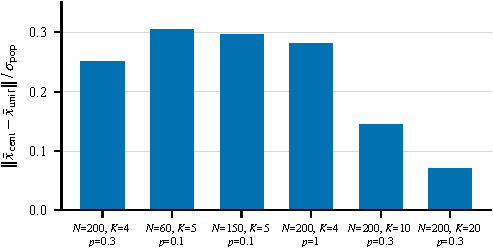
\includegraphics{fig_mechanism_magnitude}
\caption{Displacement induced by centrality weighting, in units of the
population's own spread. The mechanism moves each update by a quarter to a
third of the population spread; it is not a small correction.}
\label{fig:magnitude}
\end{figure}

Across the published and implemented settings $\rho$ ranges from $0.25$ to
$0.31$: the centrality-weighted aggregate differs from the plain neighbourhood
mean by roughly a third of the population's spread. The coefficient of
variation of betweenness over nodes is $0.65$--$0.89$, so the weights are
strongly heterogeneous rather than near-uniform.

Two predictions of Section~\ref{sec:leverage} are confirmed directly. On the
ring lattice ($p=0$), which is vertex-transitive, we measure
$\rho = 3.1\times10^{-17}$: the mechanism is inert by construction, exactly as
$\chi_i \equiv 0$ requires. And because betweenness is exactly zero at many
nodes of a sparse small-world graph, the guard $\varepsilon$ drives the
within-neighbourhood weight ratio to $O(10^{6})$--$O(10^{7})$: the operator
behaves as hard masking rather than soft weighting.

\subsection{The assignment carries no information}
\label{sec:res:placebo}

Table~\ref{tab:placebo} gives the comparison between
the published method and its permutation control.

\begin{table}[t]
\caption{\textsc{Social} against its permutation control. Paired Wilcoxon per
function with Holm correction; $\bar{\delta}$ is the mean effect over the
suite and the interval is its $90\%$ bootstrap CI. No comparison yields a
single significant difference.}
\label{tab:placebo}
\centering
\small
\setlength{\tabcolsep}{4pt}
\begin{tabular}{@{}lccccl@{}}
\toprule
Suite & $D$ & Budget & $n_f$ & W/L & $\bar{\delta}$ [90\% CI] \\
\midrule
Classic & 30 & $2.0\!\times\!10^{4}$  & 10 & 0/0 & $+0.048$ \\
Classic & 30 & $1.05\!\times\!10^{5}$ & 10 & 0/0 & $+0.078$ \\
CEC2017 & 10 & $1.0\!\times\!10^{5}$  & 28 & 0/0 & $-0.004$ $[-0.034,+0.026]$ \\
CEC2017 & 30 & $3.0\!\times\!10^{5}$  & 28 & 0/0 & $-0.010$ $[-0.038,+0.020]$ \\
CEC2017 & 50 & $5.0\!\times\!10^{5}$  & 28 & 0/0 & $-0.032$ $[-0.066,+0.002]$ \\
\bottomrule
\end{tabular}
\end{table}


On $104$ function comparisons spanning two suites, three dimensions, five
budgets and a twenty-fivefold range of evaluation counts, permuting betweenness
values across nodes changes nothing that survives correction. The largest
effect anywhere is $|\delta|=0.26$; suite means are within $\pm0.08$ of zero. A
mechanism that displaces every update by a third of the population spread can
have its node-to-score assignment randomised without measurable consequence.

The dimensional invariance is a prediction of the framework rather than an
additional observation. By \eqref{eq:leverage} the structural leverage
$\chi_i$ depends only on the graph and the score vector, not on $D$, so the
mechanism's strength---and hence what its randomisation can destroy---should
not change with dimension. Across the three protocol dimensions the suite-level
effect is $-0.004$, $-0.010$ and $-0.032$, all equivalent to zero within
$|\delta|<0.10$ and the first two within $|\delta|<0.05$.

\subsection{Equivalence, and the limits of the present design}
\label{sec:res:tost}

A non-significant difference is not equivalence, so we test the latter
directly (Section~\ref{sec:stats}). Here the answer depends on the level of
aggregation, and we report both.

At the level of the suite, equivalence holds comfortably, and tightens with
sample size. At $D=30$ with the $51$ runs the CEC2017 protocol prescribes, the
mean effect over the $28$ functions is $\bar{\delta}=-0.010$ with a $90\%$
interval of $[-0.038,+0.020]$: contained not only in the negligible band but in
the far stricter $|\delta|<0.05$. A one-sample Wilcoxon test on the
per-function effects gives $p=0.34$. At $D=10$ with $30$ runs the mean effect
is $-0.004$, interval $[-0.034,+0.026]$, likewise inside $|\delta|<0.05$.

Per function the picture is different, and the reason is worth separating into
two parts. Raising the runs from $30$ to $51$ narrows the median $90\%$
half-width from $0.181$ to $0.139$---exactly the $\sqrt{30/51}$ the sampling
theory predicts---and raises the count of formally equivalent functions from
$1$ to $6$ of $28$. It does not raise it further, because equivalence at margin
$m$ requires $|\hat{\delta}|+\text{half-width}<m$, not merely
$\text{half-width}<m$: with a median $|\hat{\delta}|$ of $0.063$, reaching
$|\delta|<0.147$ on the median function would take roughly $100$ runs. And no
sample size suffices for all of them: on $4$ of $28$ functions the estimated
effect already exceeds $0.147$, so a genuine, if small, difference is present
there. At the small-effect margin $|\delta|<0.33$, $26$ of $28$ are equivalent.

Per-function intervals are given in the supplementary material. Most sit
inside the band but cross its edge, which is the visual form of this
distinction: failing to detect a difference is not the same as establishing
its absence.


We state the conclusion at the strength the evidence supports, which is not
that the two arms are identical. Across the suite the assignment of centrality
scores to graph positions has an effect equivalent to zero within a margin four
times stricter than the negligibility threshold. Per function, effects are
bounded within a small margin, a handful are near the negligibility boundary,
and none survives correction as a difference.

\subsection{Heterogeneity does what the assignment does not}
\label{sec:res:p1p2}

Section~\ref{sec:claim} separated two properties that ablation confounds. The
data separate them too. Comparing the permutation control against uniform
mixing on the same graph isolates (P1), heterogeneity, with the assignment
already destroyed: \permcontrol{} beats \textsc{Unif}$_4$ on $3$ of $28$
CEC2017 functions ($F_{12}$, $F_{22}$, $F_{23}$; $\delta=-0.37,-0.53,-0.74$;
Holm-corrected $p\le0.013$) and loses on none. Comparing \textsc{Social}
against \permcontrol{} isolates (P2), the assignment: $0$ of $28$.

Unequal weights therefore help slightly; \emph{which} neighbour receives the
large weight does not matter at all. An ablation reports the sum of the two and
attributes it to structure. This is the confound of Section~\ref{sec:claim},
measured.

The practical consequence is immediate. Betweenness is roughly $30\%$ of
per-iteration runtime and can be replaced by any heterogeneous weighting---a
fixed random draw suffices---at no cost in solution quality.

\subsection{Calibrating the instrument}
\label{sec:res:calibration}

A null result is worth only as much as the test's ability to return a non-null
one. We therefore ran the same controls on two further mechanisms of the same
optimizer, on the same suite, at the same sample size and with the same
statistic. Fig.~\ref{fig:calibration} places the three side by side.

\emph{Fitness influence} (Section~\ref{sec:positive}) is the positive control:
the permuted score is a direct function of objective values the run has already
paid for. Permuting it does cost performance, but less uniformly than we
expected. At suite level the effect is $\bar{\delta}=-0.051$ with $90\%$
interval $[-0.117,+0.008]$, which includes zero; $17$ of $28$ functions favour
the unpermuted arm. The effect is concentrated by problem class: $-0.150$ on
the nine composition functions and $-0.152$ on the two unimodal ones, against
$+0.012$ on hybrids and $+0.016$ on simple multimodals. On $F_{23}$ it reaches
$\delta=-0.80$ with Holm-corrected $p=0.003$.

That single function settles the power question for the permutation control:
the same procedure, applied to a different score on the same optimizer, detects
an effect of $0.80$. It is not blind. Applied to the centrality assignment it
returns $-0.010$ with an interval four times inside the negligibility margin.

\emph{Adaptive selection} is the policy control applied to \textsc{Ads}, which
chooses neighbourhood degree online by sliding-window UCB on observed
improvement. Here the instrument returns a clear signal: $\bar{\delta}=-0.101$
with interval $[-0.149,-0.061]$ excluding zero, a one-sample Wilcoxon
$p=1.5\times10^{-5}$, and $24$ of $28$ functions favouring informed selection
over uniform switching.

Two points follow, and the second corrects an earlier reading of our own
results. First, the ordering across the three contrasts---null, intermediate,
clear---is exactly what a working instrument should produce, and it is produced
without any change of suite, sample size or statistic. Second, per-function
Holm correction across $28$ comparisons is conservative enough to hide a real
suite-level effect: it credits \textsc{Ads} with wins on only $3$ functions,
which reads as a weak effect, while the suite-level estimate is unambiguous.
Where a mechanism's benefit is diffuse rather than concentrated, the
per-function view understates it, and both should be reported.

\begin{figure}[t]
\centering
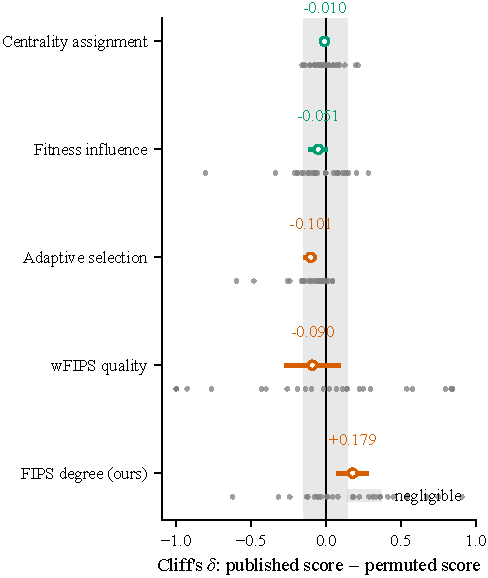
\includegraphics{fig_calibration}
\caption{The same controls on three mechanisms of the same optimizer, on
CEC2017 at $D=30$. Points are per-function effects, intervals are $90\%$
bootstrap CIs on the suite mean. The instrument separates a null mechanism from
an intermediate and a clear one without changing suite, sample size or
statistic.}
\label{fig:calibration}
\end{figure}

Mean ranks over the six arms at $D=30$ place the two sparse arms first
(\textsc{Social} $3.121$, \permcontrol{} $3.170$), then uniform mixing
($3.335$), with the density-varying arms last ($3.676$--$3.977$). That
\textsc{Social} and \permcontrol{} are adjacent, separated by $0.05$ rank units
with overlapping standard errors, is the finding of
Section~\ref{sec:res:placebo} in another form. Per-function medians and the
rank plot are given in the supplementary material.


\subsection{What density does}
\label{sec:res:density}

A sweep over $K\in\{4,8,16,32,59\}$ across $49$ problem configurations at their
native dimensions, $7{,}350$ runs, finds neighbourhood size to matter in $30$
of $49$ (Friedman $p<0.05$), with rank spreads up to $3.9$ of a possible $5$
and $p$ as small as $2\times10^{-23}$. Where it matters the effect is large;
in the remaining $19$ configurations it is undetectable.

The optimum is problem- and dimension-dependent. Ruggedness, measured as the
lag-one autocorrelation of fitness along a random walk and therefore computable
online, correlates with the preference for dense neighbourhoods at
$\rho_{s}=-0.61$ ($p=3.7\times10^{-4}$) over the configurations where density
matters (supplementary material).

That correlation is carried largely by the three most rugged
functions, and it vanishes at $D=10$ ($\rho_{s}=-0.15$, $p=0.63$) while holding
at $D=30$ ($-0.73$) and $D=50$ ($-0.63$). \textsc{Penalized} and
\textsc{Penalized2} are clear counterexamples, smooth by the proxy yet
preferring the densest neighbourhood at every dimension.

Density is thus consequential, not predictable in advance from this
descriptor, and not constant across dimension---an argument for adapting it
rather than fixing it by a topology prior, and simultaneously an argument
against predicting it from landscape features.


\section{A Second Target}
\label{sec:target2}

A single audit says something about one algorithm. Whether the instrument
discriminates, and whether the pattern generalises, needs a second target from
a different family. We take the fully informed particle swarm
(FIPS)~\cite{mendes2004fully}, whose published variants distribute a fixed
budget $\phi$ among a particle's neighbours in proportion to a per-neighbour
score. This is the same construction as \eqref{eq:W} in a velocity-based
rather than a diffusion-based optimizer, so the controls transfer unchanged.

We audit \emph{w}FIPS, the published variant that weights each neighbour's
contribution by the quality of its personal best. The topology is
Barab\'{a}si--Albert rather than a regular lattice: on a regular graph every
degree is equal, $\chi_i$ of \eqref{eq:leverage} is identically zero, and a
control would be vacuous by construction rather than by measurement.

Two preconditions were checked before the comparison. The mechanism is active:
the displacement it induces is $\rho=0.22$, against $0.25$--$0.31$ for the
first target, so the two controls neutralise mechanisms of comparable
strength. And \emph{w}FIPS is not distinguishable from plain FIPS in our setup
($\bar{\delta}=+0.043$, $[-0.065,+0.150]$, $p=0.64$), consistent with the
original report that the weighting variants gave no clear gain; this matters
because it is what makes the next result surprising.

\subsection{Large effects that cancel}
\label{sec:target2:result}

At suite level the quality weighting is indistinguishable from its permutation:
$\bar{\delta}=-0.090$ with a $90\%$ interval of $[-0.278,+0.098]$, $p=0.52$,
equivalent to zero only at the small-effect margin $|\delta|<0.33$. Read from
that line alone, the conclusion would be the same as for centrality.

It is not the same. The per-function view (Fig.~\ref{fig:calibration}, fourth
row) shows $13$ of $28$ functions with $|\delta|>0.5$ and $15$ surviving Holm
correction, in \emph{both} directions. Permuting the quality scores is
catastrophic on $F_4$, $F_6$, $F_7$, $F_9$ and $F_{17}$---$\delta=-1.00$,
every paired run, $p=2\times10^{-9}$---and significantly \emph{helpful} on
$F_8$, $F_{21}$, $F_{24}$ ($\delta\approx+0.85$). The effect sorts by problem
class: mean $\delta$ is $-0.431$ on the simple multimodal functions and
$-0.320$ on the hybrids, where permuting hurts, against $+0.314$ on the
compositions and $+0.434$ on the unimodal pair, where it helps.

So the score carries a great deal of information, and the information is
good on some landscape classes and actively misleading on others. Learning
preferentially from the better neighbours helps where the neighbourhood's
quality ordering predicts which direction is worth following, and hurts where
it concentrates the swarm on an incumbent basin---which is what the sign flip
between simple multimodal and composition landscapes describes.

\subsection{Two ways a single view misleads}
\label{sec:target2:views}

The two targets fail the same suite-level test for opposite reasons, and the
contrast is the methodological point.

For centrality, the per-function effects are small everywhere: nothing
happens, anywhere. For quality weighting, the per-function effects are large
almost everywhere and cancel in the mean: a great deal happens, in both
directions. A suite mean alone calls both ``no effect''.

The mirror-image failure appeared in our own adaptive scheme
(Section~\ref{sec:res:calibration}): there the per-function view under Holm
correction credited only $3$ of $28$ wins and read as a weak effect, while the
suite-level estimate was unambiguous ($\bar{\delta}=-0.101$,
$p=1.5\times10^{-5}$, $24$ of $28$ in its favour). Correction across $28$
comparisons is conservative enough to hide a benefit spread thinly over a
suite.

Neither view is sufficient and neither is wrong. A benefit that is diffuse
survives aggregation and not correction; a benefit that is concentrated and
sign-varying survives correction and not aggregation. We report both
throughout and would encourage the same, because each of the two failures is
demonstrated here on real data rather than argued in principle.

\subsection{A synthetic mechanism, for contrast}
\label{sec:target2:synthetic}

The published FIPS family weights by quality or by distance; there is no
degree-weighted member. We constructed one---$w_n=\deg(n)$ on the same
scale-free graph---not as an audit of anyone's claim but to check that the
instrument reports a harmful mechanism as harmful rather than merely as
non-null. It does: $\bar{\delta}=+0.179$ with interval $[+0.074,+0.283]$,
$p=0.014$, and the ablation is better still, uniform weighting beating degree
weighting by $\bar{\delta}=+0.452$ at $p=1.5\times10^{-7}$. Concentrating
influence on the hubs of a scale-free graph accelerates consensus and costs
diversity, which is the mechanism $\chi_i$ measures: degree weighting has the
largest leverage of any scheme we tested ($\chi=0.52$ against $0.40$ for
quality).

Taken together the instrument now separates five outcomes on one suite with
one statistic: inert by construction (a vertex-transitive topology),
active but uninformative (centrality), informative with class-dependent sign
(quality), uniformly harmful (degree), and uniformly beneficial (adaptive
density). A null returned by a test with that range is a statement about the
mechanism.

\section{Discussion}
\label{sec:discussion}

\subsection{How a mechanism can be active and uninformative at once}

The two findings that look contradictory---displacement of a third of the
population spread, and complete insensitivity to permutation---are reconciled
by \eqref{eq:leverage}. The displacement is governed by $\chi_i$, which depends
only on how \emph{concentrated} the weights are, not on where the concentration
falls. Betweenness on a sparse small-world graph is highly dispersed and
exactly zero at many nodes, so $\chi_i$ is large; the guard $\varepsilon$ then
makes the operator behave as hard masking, excluding a subset of neighbours
from each aggregate. Permuting the scores changes \emph{which} neighbours are
excluded but not \emph{how many}, leaving $\chi_i$ statistically unchanged.

What this says about the mechanism is specific: it perturbs the neighbourhood
aggregate strongly, and the perturbation is effectively a structured random
subsampling of neighbours. Subsampling neighbours has an effect---it is the
(P1) contribution we measure at $3$ of $28$ functions---but the identity of the
retained neighbours does not, because betweenness on a graph whose edges bear
no relation to the objective landscape cannot be related to the landscape
either. The graph is a small-world prior fixed before the first evaluation;
nothing in the search updates it toward the problem.

This suggests where a structural mechanism could genuinely carry information,
and it is not in the weighting but in the graph. A topology derived from the
landscape---edges reflecting estimated barrier heights or basin membership
rather than a Watts--Strogatz prior---would make betweenness a statement about
the search space rather than about an arbitrary lattice. Local optima
networks~\cite{ochoa2008lon} build exactly such graphs, but offline and for
characterisation; the wider landscape-analysis literature~\cite{malan2021survey}
is likewise diagnostic rather than generative. Whether an online estimate is accurate enough to drive
search is open, and the controls developed here are the instrument that would
settle it: the prediction is that on a landscape-derived graph, unlike the one
tested, permutation would hurt.

\subsection{A practical consequence}

Betweenness centrality is roughly $30\%$ of per-iteration runtime in the
reference implementation, and computing it costs $O(N\!\cdot\!M)$. Our results
say it can be replaced by any heterogeneous weighting---a fixed random draw
suffices---with no measurable loss, and by uniform weighting at a cost of about
$0.17$ rank units on the CEC2017 suite. For practitioners the recommendation is
concrete: if a centrality-weighted method is used, compute the cheapest
centrality available, or none.

\subsection{Density is the component that survives, and it resists prediction}

Of the structural choices we examined, neighbourhood size is the one with a
large and reproducible effect: consequential in $30$ of $49$ configurations,
with rank spreads up to $3.9$ of $5$. It is also the one the literature has
studied longest, from Kennedy and Mendes~\cite{kennedy2002population} through
the cellular-EA ratio~\cite{alba2005exploration}. Our contribution here is
negative and specific: the optimum is not predictable in advance from a
landscape ruggedness descriptor. The correlation is moderate
($\rho_{s}=-0.61$), carried by a few functions, absent at $D=10$, and
contradicted outright by the penalised functions.

That negative result is what motivated an adaptive scheme rather than a
predictive one, and it is worth stating why the distinction matters. A
predictor must be right about the landscape; an adaptive rule need only be
right about which of a few alternatives is currently doing better. The second
is a far weaker requirement, and our results suggest it is the achievable one:
the predictive route fails at $D=10$ and on the penalised functions, while the
adaptive route beats its own randomisation on $24$ of $28$ functions.

\subsection{On applying the instrument to our own proposal}

We built \textsc{Ads} and subjected it to the same policy control we would ask
of anyone else. It passes: informed selection beats uniform switching over the
same densities by $\bar{\delta}=-0.101$, $p=1.5\times10^{-5}$, on $24$ of $28$
functions, so the benefit is not merely from varying density, which both arms
share.

Reaching that conclusion required correcting our own first reading. Under
per-function Holm correction \textsc{Ads} wins on $3$ of $28$, which we
initially took for a weak effect; correction across $28$ comparisons is
conservative, and a benefit spread thinly across a suite fails it while being
obvious in aggregate. The diagnostic is the direction count, visible only when
the suite is the unit of analysis. Section~\ref{sec:target2:views} gives the
mirror case.

The contrasts together also say something about the optimizer under study. Its
two weighting mechanisms are null and weak at suite level, while the structural
choice that is not a weighting---how many neighbours each agent sees---carries
a clear effect. The information here lives in the coarse topology, not in the
scores computed on it.

\subsection{Implications for evaluation practice}

The confound we identify is structural, not incidental. Whenever a component
both alters the operator and is claimed to carry information, ablation reports
the sum of the two effects and the claim is attributed the whole. The remedy is
cheap: a permutation of the values the component consumes, or a randomisation
of the policy it implements, costs one additional arm and no additional budget
per arm. We would encourage reporting it wherever a structural or adaptive
claim is made, in the same way that effect sizes and non-parametric tests have
become expected.

Two caveats belong with that recommendation. First, a control is only
interpretable if the mechanism is active, which is why we report $\rho$
alongside every comparison; on a vertex-transitive topology the comparison is
vacuous by \eqref{eq:leverage}. Second, an equivalence claim needs an
equivalence test, and adequate power for it is more demanding than it looks:
equivalence at margin $m$ requires the point estimate \emph{and} its interval
to fit inside the margin, so halving the interval width does not suffice when
the estimate itself sits near the boundary. Our own per-function claims stop
at the small-effect margin for that reason, and we say so rather than resting
on non-significance.

\section{Threats to Validity}
\label{sec:threats}

\subsection{Scope of the conclusion}

We audit one published centrality-weighted optimizer and one adaptive scheme of
our own. The controls are defined for the general form \eqref{eq:master}, and
Proposition~\ref{prop:mean} holds for any score-proportional weighting, but the
empirical finding is about these two mechanisms. Whether other structural
statistics---closeness, eigenvector centrality, PageRank---or other graph
families behave the same way is untested here. We regard this as the principal
limitation: the instrument is general, the evidence is not yet.

Two considerations bear on how far the result plausibly extends. The argument
of Section~\ref{sec:discussion} turns on the graph being fixed before the
first evaluation and unrelated to the objective, which is true of every
Watts--Strogatz-based method we are aware of. And two independently designed
mechanisms failed their controls in the same way. Neither is evidence about
methods we did not run.

\subsection{Statistical power}

The primary contrast is run at the $51$ repetitions the CEC2017 protocol
prescribes; the remaining arms and the $D=10$ suite are run at $30$, which we
note as a limitation rather than a convention.

Per-function equivalence is nonetheless not established at the negligibility
margin, and additional runs would not fully establish it. At $51$ runs the
median $90\%$ half-width is $0.139$, below the $0.147$ margin, yet only $6$ of
$28$ functions are formally equivalent, because the criterion is
$|\hat{\delta}|+\text{half-width}<m$ rather than $\text{half-width}<m$. On the
median function, reaching the negligibility margin would require roughly $100$
runs; on $4$ of $28$ the point estimate itself exceeds $0.147$, so no sample
size would place them inside that band. Our equivalence claim is therefore made
at suite level, where the interval $[-0.038,+0.020]$ is contained in
$|\delta|<0.05$, and per function we claim only that effects lie within a small
margin ($26$ of $28$ at $|\delta|<0.33$) and that none survives correction as a
difference.

This is a real limit on the strength of the negative result, and we prefer to
state it than to rest on the difference tests alone. What the data exclude is a
systematic effect of the assignment across a suite; what they do not exclude is
a small effect on particular functions.

\subsection{Construct validity of the controls}

The permutation control assumes the score multiset is the quantity to hold
fixed. If a method's benefit came from the \emph{joint} distribution of scores
and degrees---high-degree nodes systematically receiving high scores---then
permutation would break that too, and attribute to assignment something that
belongs to a degree--score coupling. We regard this as a distinction without a
practical difference here, since such a coupling is exactly the kind of
structural information the claim asserts; but a reader who separates them
should read our result as covering both.

The policy control randomises selection while preserving the switching
schedule. It therefore tests whether selection is informed, not whether the
epoch length or the arm set are well chosen. A method whose benefit lay
entirely in its schedule would pass our control while making a weaker claim
than its authors intend.

\subsection{Implementation and benchmark choices}

All arms share one implementation, which removes a large source of variance but
means an implementation-level defect would affect every arm. We verified the
vectorized update against the reference path to $8.9\times10^{-16}$ per step
and to identical run distributions before using it. Population size is fixed at
$N=60$ throughout; the density sweep varies degree but not $N$, so interactions
between the two are unmeasured.

Two CEC2017 functions are absent, $F_{2}$ by the organisers' advice and
$F_{30}$ because the reference implementation we use omits it. The protocol's
fourth dimension, $D=100$, is not run; at several times the cost of $D=50$ it
was beyond the single machine available, and we note it as unfinished rather
than unnecessary. The primary contrast is run at all three dimensions we do
report; the density and adaptive arms are run at $D\in\{10,30\}$, since the
$7{,}350$-run sweep already covers density at $D\in\{10,30,50\}$.

\subsection{Reproducibility}

Every run is stored individually, keyed by arm, function, dimension and seed,
and every figure and table is produced by a script from those files. Seeds are
shared across arms so all comparisons are paired. Runs were executed on one
machine with a fixed software environment; we report the parallel throughput
measurements that determined the scheduling, since they affect wall-clock
figures but not results.

\section{Conclusion}
\label{sec:conclusion}

Score-weighted metaheuristics are justified by a causal claim---that a
per-neighbour score, computed on the population graph or on the run's own
history, carries information about where to search---which an ablation cannot
establish, because deleting the component changes the mixing operator along
with the information it carries.

We defined two controls that keep the mechanism running at full strength and
destroy only the information it is claimed to use. Permuting a score across
nodes yields an operator equal to uniform mixing in expectation that retains
the original's weight heterogeneity in every realisation
(Proposition~\ref{prop:mean})---exactly the separation an ablation fails to
make---while a leverage bound (Proposition~\ref{prop:leverage}) states when
such a comparison is informative at all.

Applied to a published betweenness-weighted optimizer, the controls give a
clear answer. The mechanism is active, displacing each update by a quarter to a
third of the population's spread. Its assignment of scores to graph positions
is not: across $104$ function comparisons on two suites, three dimensions and
five budgets, permutation changes nothing that survives correction, and at
suite level the effect is equivalent to zero within a margin four times
stricter than negligibility. Unequal weights help slightly, on $3$ of $28$
functions; which neighbour receives the large weight matters on none.

A null result of this kind is only as good as the test's ability to return a
non-null one, so we calibrated the instrument on four further mechanisms,
unchanged in suite, sample size and statistic. Within the same optimizer it
returns an intermediate, class-dependent effect on the fitness-influence
weighting and a clear one on adaptive density selection ($\bar{\delta}=-0.101$,
$p=1.5\times10^{-5}$). On a second published optimizer, the fully informed
particle swarm, it returns a uniformly harmful effect for a synthetic
degree weighting of our own construction, and for the published quality
weighting something else again: per-function effects reaching $|\delta|=1$ in
both directions, significant on $15$ of $28$ functions, that cancel to
$\bar{\delta}=-0.090$ in the mean. Five distinguishable outcomes---inert by
construction, uninformative, sign-varying, harmful, beneficial---on one suite
with one statistic. A null returned by a test with that range is a statement
about the mechanism.

That fourth case also settles a question of reporting: centrality and quality
weighting fail the same suite-level test for opposite reasons---nothing happens
anywhere, against a great deal happening in both directions---while our own
adaptive scheme shows the mirror failure, an effect unambiguous in aggregate
that per-function correction hides. Neither view is sufficient and we report
both.

What carries information in this algorithm, then, is not the scores computed on
the graph but the graph's coarse density: consequential in $30$ of $49$
configurations, with an optimum that is problem- and dimension-dependent and
resists prediction from a ruggedness descriptor. We built an adaptive scheme on
that basis and subjected it to the second control, which it passes.

The instrument costs one arm and no additional budget, and we would encourage
its use wherever a structural or adaptive claim is made, under two conditions
our own analysis makes concrete: report the displacement, so that a control on
an inert mechanism is not mistaken for evidence, and test equivalence
explicitly with adequate power rather than resting on a non-significant
difference. The controls apply unchanged to any score-proportional weighting,
so the audit can be widened directly; the constructive extension is to ask
whether a graph derived from the landscape, rather than fixed in advance, would
make a structural statistic informative. The prediction these controls can test
is that on such a graph permutation would hurt.


\section*{Reproducibility}
All code, per-run result files, random seeds, and the scripts that produce
every figure and table in this paper are available at
\url{https://github.com/anonymerauthor/structure-placebo}. Each run is stored as an individual
record keyed by (variant, function, dimension, seed), so any single number
in the paper can be traced to the run that produced it.

\bibliographystyle{IEEEtran}
\bibliography{refs}

\end{document}
